\documentclass[]{article}
\usepackage{graphicx}
\usepackage{multirow}
\usepackage{ctex}
\usepackage{xeCJK}  
\usepackage{listings}
\usepackage{xcolor}
\usepackage{graphicx}
\usepackage{geometry}
\geometry{a4paper,left=3cm,right=3cm,top=2cm,bottom=2cm}
\lstset{
    language = C++,
    numbers=left, 
	breaklines=true,
    numberstyle= \tiny, 
    keywordstyle= \color{ blue!70},
    commentstyle= \color{red!50!green!50!blue!50}, 
    frame=shadowbox, % 阴影效果
    rulesepcolor= \color{ red!20!green!20!blue!20} ,
    escapeinside=``, % 英文分号中可写入中文
    xleftmargin=2em,xrightmargin=2em, aboveskip=1em,
    framexleftmargin=2em,
    tabsize=2
} 

\title{人工智能导论\\ 四子棋作业报告}
\author{齐强 2017011436 计75}


\begin{document}
\maketitle
\tableofcontents
\newpage
%abstract



\section{代码结构}
\begin{enumerate}
    \item {Uct.h: 包含 State Uct两个类\\
        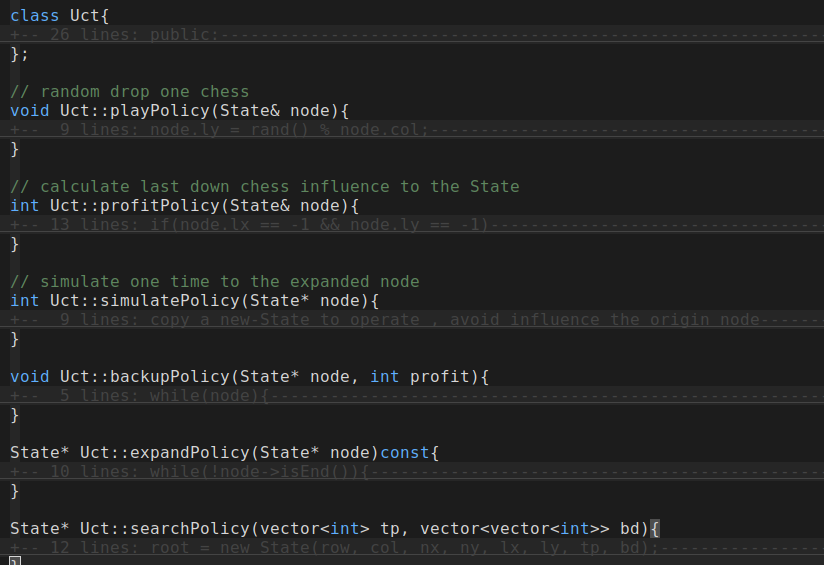
\includegraphics[scale=0.6]{pic/1.png}\\
        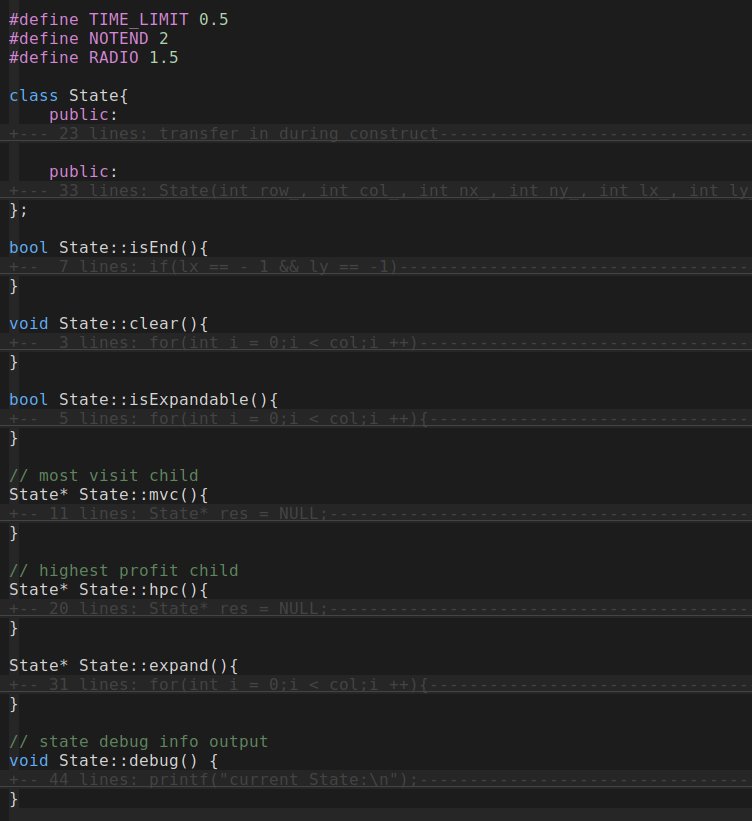
\includegraphics[scale=0.7]{pic/2.png}\\
    }
    \item{Judge.h Judge.cpp : 在给定代码基础上做了简单修改
    }
\end{enumerate}

\section{算法思路}
\begin{enumerate}
    \item 经典 “蒙特卡洛方法” + “信心上限树“算法
    \item 通过构建构建 UCT树、随机模拟对战过程、计算收益,从而确定最佳落子点
    \item {选择模拟对战节点方法:
        \begin{enumerate}
            \item 从根出发,若当前点可以扩展新的子节点,则扩展并选中新扩展的点;
            \item 若当前点无法扩展新的子节点,则选中以当前点为根的子树中profitRadio最高的叶节点
            \item profitRadio计算规则 $\frac{Q(v)}{N(v)}+c \sqrt{\frac{2 \ln (N(u))}{N(v)}}$
            \item u 为当前节点,v 为考察的子节点。N (v) 为 v 被回溯的次数,Q(v) 为 v回溯的总得分
        \end{enumerate}
    }
\end{enumerate}

\section{优化尝试}
\begin{enumerate}
    \item{
        对于常数C的调节:\\
        进行了几次实验,通过调节C的大小,根据胜率进行了几次二分实验,最后确定大概C为0.5时,效果比较好
    } 
    \item {
        对于增加模拟次数的尝试:\\
        调高模拟次数,能够显著地提高获胜概率,所做的尝试有
        \begin{itemize}
            \item 将vector改为数组(失败,代码改动较多,未能及时完成)
            \item 将二维board vector 改为一维vector(失败)
            \item 改变时间判断方法,由每模拟一次判断一次时间,改为模拟1000次判断一次时间,能够增加一些模拟次数
        \end{itemize}
    }
\end{enumerate}

\section{测试效果}
\paragraph{} 写了一些自动测试脚本,调用compete.exe 
\paragraph{} 对于前50个TestCase dll,胜率基本>0.8并接近于1\\
\paragraph{} 下面是对于90-100 dll的结果记录

\begin{center}
    \begin{tabular}{lllllll}
    \hline
    dll & 90 & 92 & 94 & 96 &98 & 100   \\ \hline
     C = 0.5 & 0.4& 0.5& 0.2 & 0.2  & 0.3                              & 0.2   \\ \hline 
     C = 0.8 & 0.5& 0.8& 0.7 & 0.2  & 0.7                              & 0.2   \\ \hline
     C = 1.5 & 0.4& 0.5& 0.7 & 0.8  & 0.3                              & 0.2   \\ \hline
    \end{tabular}
\end{center}

\section{遇到困难与解决方法}
\begin{enumerate}
    \item 对于空间问题的解决
    \item 对于expand的正确逻辑实现出现了很多问题
    \item 对于很多玄学bug,各种卡掉....
\end{enumerate}

\section{总结收获}
本次完成大作业的过程中,学习到了蒙特卡洛模拟方法、信心上限树算法\\
学习了更多的debug的技巧...
\end{document}
